\vspace{-1mm}
\section{Problem Statement}
%
% \begin{wrapfigure}{r}{0.4\textwidth} %this figure will be at the right
%     \vspace{-5mm}
%     \centering
%     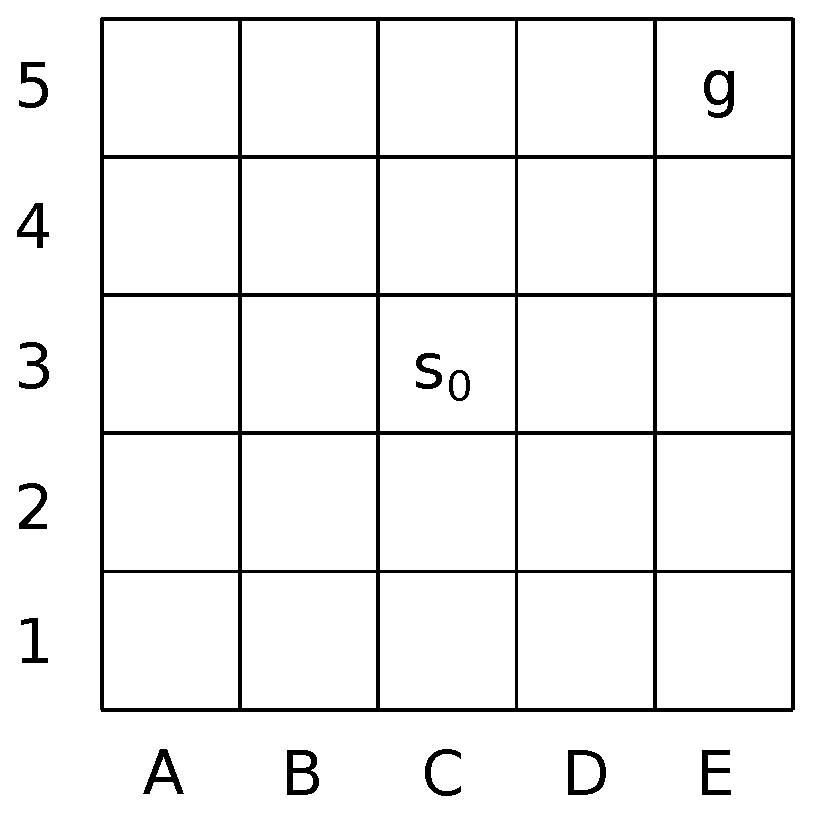
\includegraphics[width=0.25\textwidth]{./figures/drawing.eps}
%     \caption{Problemin \c{s}emati\u{g}i}
%     \label{fig:schematic}
%     \vspace{-5mm}
% \end{wrapfigure}
%
\begin{minipage}{0.5\textwidth}
    Consider the blue rectangle that shares its bottom left corner with that of
    the triangle $\triangle ABC$ as seen in the figure to the right. The length
    of the line segment between points $B$ and the top left corner of the
    rectangle is $4$ units while the length of the line segment between the
    bottom right corner of the rectangle and point $C$ is $3$  units.
\end{minipage}
\begin{minipage}{0.5\textwidth}
\begin{tikzpicture}[scale=0.85]
\tkzInit[xmax=8, ymax=8/3]
% \tkzDefPoint(0,0){B}
\tkzDefPoint(0,0){A}
\tkzDefPoint(8,0){C}
\tkzDrawTriangle[two angles = 90 and 18.43494882292201](A,C)
\tkzGetPoint{B}
\tkzLabelPoints[below left](A)
\tkzLabelPoints[below right](C)
\tkzLabelPoints[above left](B)

\tkzDefPoint(0,1){D}
\tkzDefPoint(5,0){E}
\tkzDefPoint(5,1){F}
\tkzDrawPolygon[fill=black!50!blue!20!, opacity=0.75](A,D,F,E)
% \tkzLabelPoints[below](E)
% \tkzLabelPoints[left](D)

\tkzMarkRightAngles(C,A,tkzPointResult)
\tkzDrawPoints(A,B,C)

\tkzDefPoint(5,-0.1){E1}
\tkzDefPoint(5,-0.3){E2}
\tkzDrawSegment[color=black](E1,E2)
\tkzDefPoint(8,-0.1){C1}
\tkzDefPoint(8,-0.3){C2}
\tkzDrawSegment[color=black](C1,C2)
\tkzDefMidPoint(E1,E2) \tkzGetPoint{E12mid}
\tkzDefMidPoint(C1,C2) \tkzGetPoint{C12mid}
\tkzDrawSegment[color=black](E12mid,C12mid)

\tkzDefPoint(-0.1,8/3){B1}
\tkzDefPoint(-0.3,8/3){B2}
\tkzDrawSegment[color=black](B1,B2)
\tkzDefPoint(-0.1,1){D1}
\tkzDefPoint(-0.3,1){D2}
\tkzDrawSegment[color=black](D1,D2)
\tkzDefMidPoint(B1,B2) \tkzGetPoint{B12mid}
\tkzDefMidPoint(D1,D2) \tkzGetPoint{D12mid}
\tkzDrawSegment[color=black](B12mid,D12mid)

\tkzLabelSegment[left, font=\footnotesize](B12mid,D12mid){4}
\tkzLabelSegment[below, font=\footnotesize](E12mid,C12mid){3}

\end{tikzpicture}
\end{minipage}

\begin{enumerate}
    \setlength\itemsep{0em}
    \item Find the area of the rectangle.
    \item What is the minimum area of the triangle $\triangle ABC$?
\end{enumerate}